\documentclass[conference]{IEEEtran}
\IEEEoverridecommandlockouts
% The preceding line is only needed to identify funding in the first footnote. If that is unneeded, please comment it out.
\usepackage{cite}
\usepackage[normalem]{ulem}
\usepackage{amsmath,amssymb,amsfonts}
\usepackage{algorithmic}
\usepackage{comment}
\usepackage{graphicx}
\usepackage{hyperref}
\usepackage{textcomp}
\usepackage{xcolor}
\usepackage{cite}
\usepackage{float}
\usepackage{enumitem}
%\usepackage{subfig}
\usepackage{afterpage}
\usepackage{xfrac}
\usepackage{siunitx}
\usepackage{acro}
\usepackage{url}
\usepackage{doi}
\usepackage{lettrine}
\usepackage[utf8]{inputenc}
\usepackage{fancyhdr}
\usepackage{subcaption}
\usepackage{caption}
\usepackage[ruled,vlined]{algorithm2e}


% Set the paper identifier number
%\newcommand{\paperid}{1570979187}

% Set up the fancyhdr package for all pages

%\fancypagestyle{IEEEtitlepagestyle}{
  %\fancyhf{}
  %\fancyhead[R]{\paperid}
%}

% Set up the fancyhdr package
%\fancypagestyle{plain}{
 % \fancyhf{}
  %\fancyhead[R]{\paperid}
  %\renewcommand{\headrulewidth}{0pt}
%}

% Apply the fancyhdr package to all pages
\pagestyle{plain}

\DeclareAcronym{edt}{
  short = EDT,
  long = Energy Detection Threshold
}
\DeclareAcronym{tap}{
  short = TAP,
  long = Time-Averaged Power
}
\DeclareAcronym{ecc}{
  short = ECC,
  long = Electronics Communications Committee
}
\DeclareAcronym{crtc}{
  short = CRTC,
  long = Canadian Radio-television and Telecommunications Commission
}
\DeclareAcronym{ap}{
  short = AP,
  long = Access Point
}
\DeclareAcronym{fcc}{
  short = FCC,
  long = Federal Communications Commission
}
\DeclareAcronym{cca}{
  short = CCA,
  long = Clear Channel Assessment
}
\DeclareAcronym{rf}{
  short = RF,
  long = Radio Frequency
}
\DeclareAcronym{udp}{
  short = UDP,
  long = User Datagram Protocol
}
\DeclareAcronym{usrp}{
  short = USRP,
  long = Universal Software Radio Peripheral
}
\DeclareAcronym{bpsk}{
  short = BPSK,
  long = Binary Phase Shift Keying
}
\DeclareAcronym{cs}{
  short = CS,
  long = Carrier-Sensing
}
\DeclareAcronym{lbt}{
  short = LBT,
  long = Listen-Before-Talk
}
\DeclareAcronym{mcs}{
  short = MCS,
  long = Modulation and Coding Scheme
}
\DeclareAcronym{cept}{
  short = CEPT,
  long =  European Conference of Postal and
Telecommunications Administrations
}
\DeclareAcronym{ec}{
  short = EC,
  long =  European Commission
}
\DeclareAcronym{eu}{
  short = EU,
  long =  European Union
}
\DeclareAcronym{etsi}{
  short = ETSI,
  long =  European Telecommunications Standards Institute
}
\DeclareAcronym{hs}{
  short = HS,
  long =  Harmonized Standard
}
\DeclareAcronym{rlan}{
  short = RLAN,
  long =  Radio Local Area Network
}
\DeclareAcronym{ised}{
    short = ISED,
    long  = {Innovation, Science and Economic Development Canada}
}
\DeclareAcronym{dut}{
    short = DUT,
    long = {Device Under Test}
}
\DeclareAcronym{sdr}{
    short = SDR,
    long = {Software Defined Radio}
}
\DeclareAcronym{ofdm}{
    short = OFDM,
    long = {Orthogonal Frequency Division Multiplexing}
}
\DeclareAcronym{sinr}{
    short = SINR,
    long = {Signal to Interference and Noise Ratio}
}
\DeclareAcronym{snr}{
    short = SNR,
    long = {Signal to Noise Ratio}
}
\DeclareSIUnit{\Mbps}{\sfrac{Mb}{s}}
\DeclareSIUnit{\B}{B}
\DeclareSIUnit{\dBm}{dBm}
\sisetup{mode = text}
\def\BibTeX{{\rm B\kern-.05em{\sc i\kern-.025em b}\kern-.08em
    T\kern-.1667em\lower.7ex\hbox{E}\kern-.125emX}}
\newcommand\yl[1]{\textcolor{green!80!black}{YL: #1}}   
\newcommand\gh[1]{\textcolor{red!80!black}{GH: #1}} 
\newcommand\sm[1]{\textcolor{blue!80!black}{SM: #1}}
\newcommand\ds[1]{\textcolor{magenta!80!black}{DS: #1}}
\newcommand\jb[1]{\textcolor{orange!80!black}{JB: #1}}
\newcommand\st[1]{\textcolor{brown!80!black}{SL: #1}}
\begin{document}
\thispagestyle{IEEEtitlepagestyle}
\title{Experimental Measurement of Wireless Coexistence Between Wi-Fi and Narrowband Technologies in Higher Unlicensed Bands\\
} 
\author{Stone Liu,\thanks{Department of Systems and Computer Engineering, Carleton University, Ottawa, Canada. Email: stoneliu@cmail.carleton.ca} %
\and Ioannis Lambadaris,\thanks{Department of Systems and Computer Engineering, Carleton University, Ottawa, Canada. Email: ioannis@sce.carleton.ca} %
\and Sebastian Max,\thanks{Ericsson, Germany. Email: sebastian.max@ericsson.com}%
\and David Sugirtharaj\thanks{Ericsson, Sweden. Email: david.sugirtharaj@ericsson.com}
}



\maketitle
\begin{abstract}

To evaluate the coexistence of IEEE 802.11 and Narrowband Frequency Hopping (NB FH) devices in the newly available unlicensed 6 GHz spectrum, we subject both commercial and enterprise-grade IEEE 802.11 devices to interference derived from NB FH signals. We first evaluate Wi-Fi as a transmitter by empirically measuring its ability to detect NB FH transmissions on an active channel using Clear Channel Assessment (CCA) as required by the IEEE 802.11 standards. We then evaluate Wi-Fi as a receiver by empirically measuring its ability to maintain reliable communication under concurrent NB FH interference.  In this study, Additive White Gaussian signals are used to emulate key physical layer characteristics of potential interfering signals while allowing the results to be interpreted independent of any specific technology. Additionally, these signals are transmitted by a software-defined radio, with specific time and frequency domain characteristics to emulate NB FH. Our findings provide an empirical measurement approach to evaluating coexistence and reveal several inconsistencies in device performance between vendors and between different implementations of the IEEE 802.11 standard, especially in response to narrowband transmissions.

\end{abstract}
\bigskip
\renewcommand\IEEEkeywordsname{Index Terms}
\begin{IEEEkeywords}
Wi-Fi, Coexistence, 6 GHz, Unlicensed Spectrum, Energy Detection, Clear Channel Assessment (CCA), Threshold Modification, ECC, ETSI, FCC, ISED, Frequency Hopping
\end{IEEEkeywords}

\section{Introduction}
\lettrine{T}{he} proliferation of wireless communication technologies has greatly enhanced the quality of life, enabling seamless connectivity and unprecedented access to information around the world. Wireless technologies such as Wi-Fi, Bluetooth, Zigbee, and cellular networks based on the Third Generation Partnership Project (3GPP) standards, including LTE and 5G, have become essential across diverse applications, ranging from personal devices to industrial systems. The simultaneous operation of multiple wireless technologies in the same physical environment requires careful coexistence management, especially in unlicensed frequency bands. Poorly managed coexistence can result in interference, degraded performance, and reduced communication reliability.

The unlicensed \SI{2.4}{\GHz} frequency band is becoming increasingly congested as the number of wireless devices continues to grow exponentially \cite{8024280}.  This study presents an experimental approach to evaluating the coexistence of devices operating in accordance with the IEEE 802.11 standard and technology-agnostic Gaussian signals which represent wideband and narrowband technologies. The signals are designed with carefully selected physical and MAC layer properties to emulate the behaviour of other technologies which may share the spectrum with these IEEE 802.11 devices.

One of the major motivations for this work is the introduction of new unlicensed spectrum in the 6 GHz band. Although this development increases the amount of available spectrum, for these technologies, it also introduces new challenges in terms of coexistence. Relying solely on coexistence mechanisms developed for the \SI{2.4}{\giga\hertz} band may be insufficient due to several key differences between these frequency ranges.

%This paper is an extension of our previous work presented in \cite{EDT_Regional}, where we initially investigated the impacts of federal regulations on the \ac{cca} implementation of a Cisco 3702 Access Point. Here, we extend our work to present a more general experimental assessment of the impacts of wideband and narrowband Gaussian signals on commercially available IEEE 802.11 devices. The Wi-Fi \ac{dut} is assessed as both a transmitting and a receiving station, to gain insight into channel measurement and resilience against various test signals respectively. The use of Gaussian signals allows the results to be interpreted independently of any specific technology, while providing insight into certain key parameters such as signal power, bandwidth, and duration. Due to ease of commercial access, experiments are conducted in the unlicensed \SI{5}{\giga\hertz} band, but the gained insights are relevant to discussions in \SI{6}{\giga\hertz} spectrum.

The remainder of this paper is organized as follows: Section II provides background on the specifications and federal regulations governing the unlicensed spectrum. Section III discusses related work and coexistence challenges. Section IV outlines the methodology, while Section V presents the results along with a discussion of the findings. Portions of the methodology and results in this paper incorporate material from \cite{thesis}.

\section{Background}
In this section we review the regulatory frameworks, technical standards, and key technologies that influence the implementation of IEEE 802.11 and NB FH devices. Part A of this section provides the relevant federal regulations on unlicensed spectrum usage, Part B discusses the IEEE 802.11 standards and specifications for the PHY and MAC layers.

\subsection{Regulations on Unlicensed Spectrum in the 6 GHz Band}
Governing bodies such as the \ac{fcc} and \ac{ised} play a crucial role in regulating the use of radio frequencies in North America. Recent developments have opened up portions of the \SI{6}{GHz} band for unlicensed use, providing an additional \SI{1200}{\MHz} of spectrum \cite{b1_FCC_Decision}, \cite{ised2020}. This expansion is intended to alleviate congestion in existing bands and support the growing demand for wireless connectivity.

Similarly, in Europe the \ac{ecc} of the \ac{cept} has been active in regulating the lower half of the 6 GHz band for unlicensed use \cite{b2_ECC_hs}. The \ac{ecc} decision explicitly permits narrowband signals to employ frequency hopping as a mode of operation. In light of this new unlicensed frequency spectrum, Wi-Fi has already begun deployment into the \SI{6}{\giga\hertz} band \cite{wifi6g}. However, it will not be the only technology to use this frequency as Bluetooth has also announced its intention to operate in \SI{6}{\giga\hertz} as a result of the ECC's decision \cite{bluetooth6ghz}.

Relying solely on coexistence mechanisms developed for the \SI{2.4}{\giga\hertz} band may be insufficient due to several key differences between these frequency ranges. The \SI{6}{\giga\hertz} spectrum hosts incumbent services such as fixed satellite services and point-to-point microwave links, which must be protected from interference. Regulatory bodies such as the FCC have mandated the use of Automated Frequency Coordination (AFC) systems to manage spectrum access and prevent disruptions to these essential services \cite{9165719}. Furthermore, the \SI{6}{\giga\hertz} band offers wider channel bandwidths to support high-throughput applications with stringent latency and reliability requirements, which existing coexistence mechanisms may not adequately address \cite{FCC_6GHz}.


\subsection{IEEE 802.11 PHY and MAC Layer Specifications}
The IEEE 802.11-2020 standards provide a global framework for the development and implementation of wireless local area networks (WLANs), ensuring interoperability and efficient use of the available spectrum \cite{IEEE-802.11-2020}. One important mechanism that is defined by Section 17.3.10.6 of the standard is \ac{cca}, which plays a crucial role in ensuring coexistence among various wireless technologies.  \ac{cca}, otherwise known as \ac{lbt}, is a technique used by Wi-Fi devices to determine if a communication channel is clear or busy before transmitting data to mitigate interference. According to the standard, CCA is done through two functions: energy detection and preamble detection. Energy detection checks for the presence of any radio frequency (RF) energy above a certain threshold, while preamble detection looks for Wi-Fi signals with a specific preamble. If the channel is found to be occupied by either energy or a preamble, the device defers its transmission to avoid collisions. The standard states that the energy detection mechanism shall detect the medium as busy within \SI{4}{\micro\second} of any signal with a received energy that is \SI{20}{\dB} above the most robust modulation and coding (MCS) rate sensitivity. For a \SI{20}{MHz} channel, this value is \SI{-82}{\dBm} + \SI{20}{\dB} = \SI{-62}{\dBm}, which is the specified \ac{edt}. It is important to note that although this value is fixed by the standard, implementation is left to the manufacturer. In addition, this framework is not legally binding and is not necessarily reflected in federal regulations in specific regions \cite{EDT_Regional}.

In addition to these considerations, another important factor is the frequency location of sub-carriers in Wi-Fi's \ac{ofdm} implementation. Unless otherwise specified, the \ac{mcs} used for for experimentation in this study is IEEE 802.11a Binary Phase Shift Keying (BPSK) with 1/2 code rate \cite{815305}, as this is the most robust \ac{mcs} available on these devices and provides a baseline test result that is independent of adaptive link conditions. The IEEE 802.11a OFDM scheme divides the \SI{20}{\mega\hertz} channel into 52 sub-carriers with a \SI{312.5}{\kilo\hertz} sub-carrier spacing, numbered from -26 to +26, with a null at index 0. The sub-carrier frequency floor plan is as follows:


\begin{itemize}
    \item \textbf{Data Sub-Carriers}: 48 sub-carriers are used for data transmission. 
    \item \textbf{Pilot Sub-Carriers}: 4 sub-carriers are used for synchronization and channel estimation.
    \item \textbf{DC Null}: The center sub-carrier (index 0) is omitted and filled with a null value.
\end{itemize}

In this MCS scheme, each data sub-carrier is modulated using Binary Phase Shift Keying (BPSK) and encoded with a rate 1/2 convolutional code, to improve robustness against interference and multipath effects.


\section{Related Work}
The coexistence of wireless technologies in shared frequency bands has been a significant area of research, given the increasing density and diversity of wireless devices. Although mathematical models and simulations have been extensively used to analyze coexistence mechanisms in the past, real-world experimental validation remains sparse. This gap is particularly evident as Bluetooth expands into \SI{6}{\giga\hertz}, necessitating empirical studies to assess its interaction with devices operating by the IEEE 802.11 standard. The literature review that follows explores existing research on Wi-Fi and Bluetooth coexistence across different frequency bands, discusses the theoretical vs. experimental differences, and highlights the urgent need for empirical research in the 6 GHz band.

The unlicensed \SI{2.4}{\giga\hertz} band has been a focal point of coexistence research due to the widespread adoption of Wi-Fi (IEEE 802.11) and Bluetooth (IEEE 802.15.1). Both technologies utilize the same spectrum, leading to interference, particularly in dense deployment environments. Wi-Fi uses carrier-sense multiple access with collision avoidance (CSMA/CA), while Bluetooth operates using frequency hopping spread spectrum (FHSS). Early research predominantly made use of simulation models to analyze this coexistence. For instance, the study in \cite{Radioeng_Bluetooth_WiFi} developed a Simulink-based simulation to evaluate the coexistence of Bluetooth and IEEE 802.11b/g physical layers, highlighting how simultaneous operation can degrade performance for both technologies. It should also be noted that this study does not take into consideration the adaptive frequency hopping (AFH) protocol implemented in later Bluetooth standards, which would further improve the coexistence of the two technologies. Similarly, the research efforts of \cite{IJARCCE_Bluetooth_WiFi} employed MATLAB Simulink models to investigate interference effects between Bluetooth and Wi-Fi, proposing solutions like Adaptive Frequency Hopping (AFH) to mitigate such issues. A notable empirical study by researchers at Idaho National Laboratory \cite{INL_2.4GHz_Interference} evaluated the impact of Wi-Fi on ZigBee and Bluetooth in indoor environments. Their real-world testing confirmed significant performance degradation in both ZigBee and Bluetooth when Wi-Fi was active, reinforcing concerns about simulation-based underestimation of interference. Despite these findings, limited work has extended such experimental methodologies to higher frequency bands.

Unlike \SI{2.4}{\giga\hertz}, Bluetooth does not operate in \SI{5}{\giga\hertz}. Thus, most research in this band has focused on Wi-Fi coexisting with LTE Licensed Assisted Access (LTE-LAA). LTE-LAA, introduced to utilize unlicensed spectrum for cellular traffic, led to significant interference concerns for Wi-Fi networks, prompting the adoption of Listen Before Talk (LBT) mechanisms to mitigate conflicts. For example, the work in \cite{mumtaz2017} investigates the usage of unlicensed spectrum to address spectrum shortages which cannot be overcome even with sophisticated methods to improve spectral efficiency. Moreover, the paper discusses the coexistence challenges between LTE and Wi-Fi in the unlicensed spectrum. Two main methods are proposed for ensuring fair coexistence: \ac{lbt} and duty cycle. \ac{lbt}, which is preferred by several major companies and required by regulations in regions like the EU and Japan, involves the LTE system listening to the channel prior to transmitting to avoid interference with existing Wi-Fi networks. On the other hand, the duty cycle approach divides the channel time between LTE and Wi-Fi devices to ensure fair usage, though it may lead to inflexibility and increased latency. While the paper provides a comprehensive framework and discusses the regulatory and technical challenges of coexistence, it does not present specific experimental results. Similarly, the work done in \cite{Adaptive_ET} proposes an adaptive EDT algorithm that would improve Wi-Fi's performance at the cost of License Assisted Access (LAA), and supports this with simulation results. The results also show that in scenarios where interference would have a minimal impact on throughput, coordination via the adaptive EDT provides significant losses to Wi-Fi due to inefficient transmission schemes. The proposed algorithm suggests coordination amongst transmitting stations to enhance their coexistence. The work done in \cite{edt_lte} evaluates the effects of asymmetry between the IEEE 802.11 EDT value of \SI{-62}{\dBm} and the LTE EDT value of \SI{-72}{\dBm}. This study develops a coexistence simulator in ns-3 and demonstrates that lowering the EDT value of Wi-Fi improves both the performance of Wi-Fi and LTE-LAA. From the perspective of Wi-Fi, however, this would cause the device to be increasingly sensitive to neighboring technologies, particularly in the unlicensed spectrum.

The introduction of the \SI{6}{\giga\hertz} band for unlicensed use brought new coexistence challenges, particularly with the expansion of Wi-Fi 6E, Wi-Fi 7, and potential future Bluetooth implementations. Initial research on 6 GHz coexistence has been largely theoretical, focusing on spectrum sharing policies and predicted interference models.

Monte Carlo simulations and traffic models have been used to estimate collision probabilities and network performance impacts \cite{9165719}, \cite{WiFi_Spectrum_Requirements}, but these studies rely on assumptions about propagation characteristics, traffic loads, and interference patterns that have not yet been verified through experimental research.

While theoretical models and simulation-based studies have provided valuable insights into coexistence mechanisms, they inherently rely on simplified models with varying degrees of assumptions that do not fully capture the complexities of real-world wireless environments. These approaches often overlook practical factors such as hardware imperfections, environmental variability, dynamic interference patterns, and unpredictable user behavior. Furthermore, simulation-based approaches typically assume idealized traffic distributions and synchronization mechanisms, which can lead to overly optimistic findings. Without empirical validation, there remains a significant risk that regulatory policies, coexistence strategies, and spectrum-sharing mechanisms based purely on theoretical analyses may fail to perform as expected in practical deployments.

In contrast, experimental research provides ground truth validation by directly measuring coexistence performance under real-world conditions. Empirical studies allow researchers to capture non-ideal interference effects, evaluate the impact of heterogeneous traffic loads, and assess how coexistence mechanisms operate on commercial hardware rather than idealized models. While experimental studies pose challenges such as higher cost, limited scalability, and reproducibility concerns, they remain essential for refining theoretical models, informing regulatory decisions, and ensuring that future unlicensed wireless technologies can coexist harmoniously. Thus, our goal is to introduce a novel experimental measurement approach to assessing the coexistence of commercially available off-the-shelf Wi-Fi devices with narrowband frequency-hopping (NB-FH) technologies. By prioritizing direct tests via actual measurements, our aim is to mitigate the simplification bias inherent in theoretical and simulation-based studies, ensuring a more accurate evaluation of real-world coexistence challenges.


\section{Methodology}
This section focuses on the methodology used for the experiments conducted in this study. Part A details the testbed and measurement setup, and Part B discusses the generation of the Gaussian signals used for the coexistence tests.

\subsection{Testing and Measurement Setup}
In this study, we evaluate two distinct Devices Under Test (DUTs) operating according to the IEEE 802.11 standard, referred to as DUT-1, and DUT-2. These devices are enterprise and commercial grade respectively, and have unique chipsets and manufacturers. Further detail of the characteristics and settings of these devices is detailed throughout this section.

To assess the coexistence of these IEEE 802.11 DUTs with NB FH wireless technologies, the two need to be transmitted over the same wireless link at the same carrier frequency. By modifying the test setup, the \ac{sdr} generated signal can be sent to either the Wi-Fi transmitting station or the Wi-Fi receiving station to assess Wi-Fi's \ac{lbt} mechanism and reception robustness respectively. The two measurement setups are shown in Fig. \ref{pic:testbed}.

\begin{figure*}
    \begin{subfigure}{0.45\textwidth}
        \includegraphics[width=8cm]{tx_testbed.png}
        \centering
        \caption{SDR generated interference inserted to transmitter station.}
        \label{pic:tx_testbed}
    \end{subfigure}
    \hfill
    \begin{subfigure}{0.45\textwidth}
        \includegraphics[width=8cm]{rx_testbed.png}
        \centering
        \caption{SDR generated interference inserted to receiver station.}
        \label{pic:rx_testbed}
    \end{subfigure}
    \caption{Testbed block diagrams.}
     \label{pic:testbed}
\end{figure*}

DUT-1 is unique in that it provides a high level of control over the device's parameter settings, and enables monitoring of live radio traffic statistics. DUT-2 is selected as a comparative device for testing with a different chipset manufacturer. DUT-2 also has compability with OpenWRT, allowing for some level of modifiabilility.

The transmitting Wi-Fi station, referred to as the access point (1), is placed inside a \ac{rf} Isolation Chamber (12) to shield it from ambient interference. This is done for both transmitter side and receiver side tests as the antennas are designed to be sensitive to low energy signals for \ac{cca}. Due to space constraints, an RF isolation chamber is not used on the Wi-Fi node acting as the receiver (2). The coaxial cables provide sufficient shielding against ambient interference, as the nominal throughput in the absence of our SDR-generated traffic remains steady over long periods of time without significant fluctuation.

RF power combiners at (6) and (13) are used to combine transmissions from the Wi-Fi devices' multiple antennas; the insertion loss of this component is accounted for proportionate to the number of antenna ports at the Wi-Fi device. To run the experiments, iPerf3 \cite{iperf3-docs} is used to send User Datagram Protocol (UDP) traffic from a client at Linux PC-1 (2) to a server at Linux PC-2 (3). UDP traffic is chosen instead of Transmission Control Protocol (TCP) traffic to ensure that there are minimal transport layer protocol considerations in the tests, thereby isolating the effects of interference to layer-2 protocols such as medium access control and error detection. The load offered to this link is fixed, such that there is a nominal throughput of 90\% from client to server under zero-interference conditions to avoid under-utilization of the link. This ensures maximal duty-cycle conditions for the Wi-Fi transmissions, to properly assess the impacts of interfering traffic. Additionally, the size of each UDP packet is fixed to \SI{1470}{\B} to adhere to the standard packet size as prescribed by the iPerf3 documentation.

For DUT-1, an identical device with the same chipset and manufacturer is used as its companion to establish a four-hop bridge mode connection from PC-1 to PC-2. For DUT-2, a secondary device with OpenWRT compatibility is used as a companion device. Due to firmware compatibility issues with OpenWRT between devices with differing vendors, in this latter setup, the iPerf3 server is run directly on the Wi-Fi receiving device (4) instead of on PC-2. The CPU usage of the device during this is measured to be less than 1\%, indicating that this does not require extraneous computational overhead in performing Address Resolution Protocol (ARP) at higher layers. This modification from our work in \cite{EDT_Regional} allows the Wi-Fi DUT to be assessed as both a transmitter and a receiver.

The power level received at (4) can be modified by using the tunable attenuator in (9). Unless otherwise specified, the power level at the receiver is fixed to \SI{-50}{\dBm} to ensure a sufficient \ac{snr} for testing. To measure the power level of the received transmissions at (4), prior to each experiment a high-performance signal analyzer (11) is positioned such that it receives the same signal as (4). This is then used to capture the beacon frame transmissions using the signal analyzer's maximum hold feature. As shown in Fig. \ref{pic:tx_testbed}, a \SI{30}{\dB} attenuation is placed between (8) and (11) to protect the signal analyzer from high power transmissions while monitoring the channel.

Testing is conducted in the unlicensed \SI{5}{\giga\hertz} band due to the wider commercial availability of compatible Wi-Fi hardware. However, the resulting insights remain applicable to coexistence scenarios in the unlicensed \SI{6}{\giga\hertz} band, which shares similar propagation characteristics and regulatory context. Wi-Fi's channel 36 is selected for these experiments. This is a \SI{20}{\mega\hertz} Wi-Fi channel with a center frequency of \SI{5180}{\mega\hertz}. A pre-generated signal is transmitted from a \ac{sdr} device (5) onto the channel at the same carrier frequency as the ongoing Wi-Fi transmission. A tunable attenuator (10) is used to modify the power level of the SDR transmitted signal. Through careful orientation of the RF splitters, the SDR transmitted signal can be inserted either to the transmitting Wi-Fi node as shown in Fig. \ref{pic:tx_testbed}, or to the receiving Wi-Fi node as shown in Fig. \ref{pic:rx_testbed}. The power level of the SDR generated signal is increased in increments of \SI{1}{\dB} until the connection is lost, using throughput as the primary metric to ascertain the impact of interference. Additional metrics are collected with DUT-1 to distinguish device backoff due to \ac{lbt} from packet corruption and loss. The device allows for monitoring of live traffic statistics in \SI{5}{\second} intervals. In the case of device backoff, a decline in throughput should be not be accompanied by an increase in the number of packet retries. In the case of packet loss, the number of packet retries should increase proportional to any observed throughput loss. For reference, the number of successful transmissions in a \SI{5}{\second} window is about 2200 packets, with 0 retries when there is no test signal present on the channel. An additional setting for the receiver-side tests is that the node serving as the access point is set to dissociate on low acknowledgement where applicable. Both DUTs are set to have a North American parameter carrier set, and where applicable, any \ac{edt} parameters \cite{EDT_Regional} are set to \SI{-62}{\dBm} in accordance with the IEEE 802.11-2020 standards. It is important to emphasize that while a signal analyzer is employed and all insertion losses in the testbed are meticulously accounted for, the power measurements are conducted on a best-effort basis. The primary objective of this study is to evaluate the relative performance between wideband and narrowband traffic, as well as to assess device-to-device performance in a comparative manner.

The generation of these pre-generated SDR signals is detailed in the following subsection.

\subsection{Generation of Technology-Agnostic Gaussian Signals}
In this study, Gaussian signals play the role of NB FH transmissions for the assessment of coexistence with IEEE 802.11 devices. This allows for a technology-agnostic study while still maintaining key properties of interest such as bandwidth, power, dwell time and duty cycle. MATLAB was deployed to construct these signals prior to the SDR transmission, the process for generating the signal is outlined in Algorithm 1.


\begin{algorithm}[h]
\caption{Gaussian Signal Generation with Dwell Time, Duty Cycle, and Upsampling}
\label{alg:signal_generation}
\KwData{Bandwidths $BW = \{0.3125 \, \text{MHz}, 2 \, \text{MHz}, 20 \, \text{MHz}\}$}
\KwData{Dwell times $DT = \{100 \, \mu s, 1000 \, \mu s, 5000 \, \mu s, 7500 \, \mu s\}$}
\KwData{Duty cycles $DC = \{0.1, 0.5, 1.0\}$}

\ForEach{$BW$ \textbf{in} bandwidths}{
    Set sampling frequency: $fs \gets BW$\;
    Set shortest dwell time: $T_{\text{shortest}} \gets 100 \, \mu s$\;
    Calculate building block length: $L \gets T_{\text{shortest}} \times fs$\;
    
    Generate real part of signal: $x_{\text{real}} \sim \mathcal{N}(0,1)$ of length $L$\;
    Generate imaginary part of signal: $x_{\text{imaginary}} \sim \mathcal{N}(0,1)$ of length $L$\;
    Form complex signal: $x \gets x_{\text{real}} + j \times x_{\text{imaginary}}$\;

    \ForEach{$T_{\text{dwell}}$ \textbf{in} dwell times}{
        Calculate repeats: $R \gets \frac{T_{\text{dwell}}}{T_{\text{shortest}}}$\;
        Repeat signal to match dwell time: $x_{\text{on}} \gets \text{Repeat}(x, R)$\;
        
        \ForEach{$D_C$ \textbf{in} duty cycles}{
            Calculate total duration: $T_{\text{total}} \gets \frac{1}{D_C} \times \frac{\text{length}(x_{\text{on}})}{fs}$\;
            Calculate off duration: $T_{\text{off}} \gets T_{\text{total}} - \frac{\text{length}(x_{\text{on}})}{fs}$\;
            Create off portion: $x_{\text{off}} \gets \text{Zeros}(T_{\text{off}} \times fs)$\;
            Concatenate on and off portions: $x_{\text{combine}} \gets [x_{\text{on}}, x_{\text{off}}]$\;

            Normalize signal: $x_{\text{normalized}} \gets \frac{x_{\text{combine}}}{\max(\lvert x_{\text{combine}} \rvert)}$\;

            Upsample to 20 MHz: $x_{\text{upsample}} \gets \text{Resample}(x_{\text{normalized}}, 20 \, \text{MHz}, fs)$\;
            
            Save signal: Save $x_{\text{upsample}}$ to file with name based on $BW$, $T_{\text{dwell}}$, and $D_C$\;
        }
    }
}

\end{algorithm}
In this study, we generate Gaussian signals with bandwidths of \SI{312.5}{\kilo\hertz}, \SI{2}{\mega\hertz}, and \SI{20}{\mega\hertz} signals. Additionally, since NB FH is a permitted mode of operation in the unlicensed band, on-off traffic can be generated to emulate this behaviour. The "off" time of this signal can be considered equivalent to transmission on a separate frequency outside the range of the Wi-Fi channel's occupied bandwidth. This is done by generating a \SI{2}{\mega\hertz} signal using \SI{100}{\micro\second}, \SI{1}{\milli\second}, \SI{5}{\milli\second} and \SI{7.5}{\milli\second} dwell times and 10\%, 50\% and 100\% duty cycles for the \SI{2}{\mega\hertz} signals. Dwell time is defined as the amount of time the signal is active on the channel in one cycle, and duty cycle is the percentage of time the signal is active in one cycle. In this context, a cycle refers to the complete duration of one transmission-on and transmission-off sequence of the signal, as defined by the dwell time and duty cycle. This cycle is transmitted in a continuous loop by the SDR.


For each desired bandwidth, the sampling frequency of the baseband complex signal is set equal to the target passband bandwidth (BW). Since complex baseband signals are symmetric around DC (i.e., they occupy both positive and negative frequencies), this ensures that, upon modulation by the SDR onto a carrier frequency (e.g. \SI{5180}{\mega\hertz}), the resulting real-valued passband signal occupies the correct bandwidth centered around the carrier frequency. The spectral content of the baseband signal extends up to \(\pm \frac{\text{BW}}{2}\), which maps to a total bandwidth of \(\text{BW}\) at passband after upconversion.


A base Gaussian building block is generated for each of these desired bandwidths. To do this, the length of the fundamental signal block, $L$, is determined first. The building block length is the number of samples required to generate a signal that spans the minimum dwell time, $T_{\text{shortest}}$, in the array, \SI{100}{\micro\second}. By multiplying the shortest dwell time by the sampling frequency, the number of samples required for this specific time duration is determined. This block length can be expressed as:
\begin{equation}
L = T_{\text{shortest}} \cdot f_{\text{s}}
\end{equation}



The purpose of this calculation is to ensure that the generated signal has the correct number of samples to represent the desired duration for a given signal bandwidth.

With the building block length determined, the real and imaginary components of the Gaussian signal are generated using the ``randn"  function in MATLAB. This function generates random values from a standard normal distribution. Specifically, the function is used to create two sets of random numbers: one for the real part and one for the imaginary part of the signal. The input to the ``randn" function is the previously calculated block length, which directly defines how many samples are produced. This ensures that the generated real and imaginary components have exactly the same number of samples, corresponding to the number needed to span the 100 µs dwell time. The resulting vectors of real and imaginary values are combined to form the complex baseband signal. In Algorithm 1, the generation of the real and imaginary components follow a standard Gaussian distribution as follows:

\begin{align}
    x_{\text{real}} = \mathcal{N}(0,1), \quad x_{\text{imaginary}} = \mathcal{N}(0,1)
\end{align}

These real and imaginary components are then combined to form the complex signal as follows:

\begin{align}
    x(t) = x_{\text{real}}(t) + j \times x_{\text{imaginary}}(t)
\end{align}

To achieve the other desired dwell times, the previously generated base signal, with a minimal dwell time of \SI{100}{\micro\second} is repeated. The repetition process ensures that the signal maintains the same spectral and statistical properties. For instance, if the dwell time is set to \SI{1}{\milli\second}, the base signal is repeated ten times to fill this duration.

In addition to varying the dwell time, the duty cycle of the signal is modified. The duty cycle is defined as the proportion of time that the signal is active (``on") versus the total period of the signal (which includes both ``on" and ``off" times). In this study, three duty cycles are used: 10\%, 50\%, and 100\%. Fig. \ref{pic:time_sample} shows a visualization of a signal with a \SI{100}{\micro\second} dwell time and a 10\% duty cycle.
\begin{figure}[h]
    \includegraphics[width=6cm]{Time_domain_on_off.png}
    \centering
    \caption{Time-domain representation of Gaussian signal with a \SI{100}{\micro\second} dwell time and a 10\% duty cycle.}
    \label{pic:time_sample}
\end{figure}


To implement this, after constructing the ``on" portion of the signal (i.e., the repeated base signal for the desired dwell time), the ``off" portion is done through zero padding, with a length calculated based on the specified duty cycle. The total duration of the signal is computed as the inverse of the duty cycle multiplied by the duration of the ``on" portion. For example, with a duty cycle of 10\%, the ``on" portion would be followed by an ``off" portion, making the total duration ten times longer than the ``on" portion. The complete signal is then formed by concatenating the ``on" and ``off" periods. This process allows for the emulation of various NB FH transmission patterns, where the signal is periodically active and inactive.

After constructing the signal with the desired dwell time and duty cycle, normalization is performed to ensure that the signal has a consistent amplitude across all configurations. This step is important because signals with different bandwidths, dwell times, and duty cycles may have varying power levels, which could introduce inconsistencies in the analysis or real-world system performance. Furthermore, this avoids clipping when transmitted over the SDR. The normalization process involves scaling the entire signal such that its maximum absolute value becomes unity. Mathematically, this can be expressed as:

\begin{align}
x_{\text{normalized}}(t) = \frac{x(t)}{\max \lvert x(t) \rvert}
\end{align}

where \(x(t)\) represents the original signal, and \(\max \lvert x(t) \rvert\) is the maximum absolute value of the signal. By dividing the signal by this value, the resulting normalized signal \(x_{\text{normalized}}(t)\) has its peak value constrained to 1. This ensures that the amplitude of the signal is consistent, regardless of the bandwidth or the repetition applied in earlier steps.

The final step in the signal generation process is upsampling the signal to a fixed sampling rate of 20 MHz using Matlab's ``resample" function. Upsampling is required when the generated signal's bandwidth is lower than the desired final sampling frequency. In this case, since the initial signal bandwidths vary, the upsampling process ensures that the signal can be correctly transmitted on the SDR which is set at a sampling rate of \SI{20}{\mega\hertz}. To efficiently handle this interpolation process, the resample function employs a polyphase implementation which optimizes the computational workload, making it feasible to accurately upsample the signal from the original sampling frequency to \SI{20}{\mega\hertz} while maintaining signal integrity and quality. The upsampled signals are then saved in binary format for transmission via the SDR. 


The time and frequency domain properties of these signals are confirmed by using a second SDR device as a receiver. The transmitting SDR is connected directly to the receiving SDR over coaxial cable with a small amount of attenuation inserted in between the two devices for protection. The receiving SDR is able to receive a short duration the transmissions and save the data to a binary file which can be read, interpreted and plotted in MATLAB. As an example, the time-domain and Power Spectral Density (PSD) representation of a \SI{2}{\mega\hertz} test signal with a \SI{100}{\micro\second} dwell time and 10\% duty cycle are shown in Fig.  \ref{pic:PSD_sample}. As mentioned, in the time-domain, the amplitude of the signal is normalized so it ranges from -1 to 1. In the frequency domain, the PSD representation is illustrative of the signal's frequency characteristics such as bandwidth and steep out-of-band cut-off. The PSD value shown, denoted in dBm/Hz, is indicative, as it will be modified by the gain of the SDR and variable attenuators in the testbed.


\begin{figure}[h]
    \includegraphics[width=6cm]{PSD_matlab.png}
    \centering
    \caption{PSD representation of \SI{2}{\mega\hertz} Gaussian signal.}
    \label{pic:PSD_sample}
\end{figure}


Additionally, NB FH is one permitted mode of operation in the new unlicensed portions of the \SI{6}{\giga\hertz} spectrum.  To emulate a more dynamic type of frequency hopping beyond on-off traffic, the carrier frequency of the SDR device transmission is modified in real-time through a python script. The algorithm for selecting the carrier frequency is modified to alternate between \SI{5175}{\mega\hertz}, \SI{5180}{\mega\hertz} and \SI{5185}{\mega\hertz}. A delay of \SI{7.5}{\milli\second} is set so that the dwell time of the signal at each frequency is fixed. In between switching frequencies, the signal will hop out to \SI{5250}{MHz} for \SI{61.5}{\milli\second}, with an additional \SI{3}{\milli\second} overhead introduced when switching carrier frequencies where there is no transmission, totaling to an equivalent out-of-channel time of \SI{67.5}{\milli\second}. This emulates a frequency hopping signal that has a dwell time of \SI{7.5}{\milli\second} on one of the three in-channel frequencies specified, and a duty cycle of 10\%. The algorithm to generate this narrowband frequency hopping signal is defined in Algorithm 2.

\begin{algorithm}[h]
\caption{Frequency Hopping Algorithm}
\SetAlgoLined
$In\_band\_freq \gets \{5175, 5180, 5185\}$ MHz\;
$Out\_band\_freq \gets 5250$ MHz\;
$freq\_index \gets 0$\;

\While{true}{
    $carrier\_freq \gets In\_band\_freq[freq\_index]$\;
    set $current\_freq \gets carrier\_freq$\;
    \textbf{sleep}(7.5 ms)\; \tcp{In-band frequency for 7.5 ms}

    $carrier\_freq \gets Out\_band\_freq$\;
    set $curr\_freq \gets Out\_band\_freq$\;
    \textbf{sleep}(61.5 ms)\; \tcp{Out-of-band frequency for 61.5 ms}

    \eIf{$freq\_index > 2$}{
        $freq\_index \gets 0$\;
    }{
        $freq\_index \gets freq\_index + 1$\;
    }
}
\end{algorithm}



\section{Results and Analysis}
This section details the results of our coexistence testing. Part A discusses the impacts of transmitting the Gaussian signal over SDR to the Wi-Fi transmitting station, assessing its ability to perform \ac{lbt} on signals of varying powers and bandwidths. Part B discusses the impacts of transmitting the Gaussian signal over SDR to the Wi-Fi receiving station, assessing the robustness of IEEE 802.11 transmissions to different forms of interference.

\subsection{Insertion of Gaussian Signal to Wi-Fi Transmitter}
To assess the \ac{edt} of the two IEEE 802.11 DUTs, the SDR is used to transmit narrow and wideband Gaussian traffic to the Wi-Fi transmitter. Throughput is used to gauge the \ac{lbt} mechanism of these devices, noting that the nominal throughput without SDR traffic on the channel is set to 90\% as discussed in the previous section. A baseline test is conducted to determine the default EDT of the two DUTs in response to narrow and wideband signals. To do this, \SI{2}{\mega\hertz} and \SI{20}{\mega\hertz} signals are transmitted by the SDR onto a carrier frequency of \SI{5180}{MHz}, the centre of the active Wi-Fi channel. The signals are transmitted with a full duty cycle of 100\%. The results of this baseline test for DUT-1 and DUT-2 are shown in Fig. \ref{pic:Cisco_EDT_TP_Default}, and Fig. \ref{pic:Netgear_EDT_TP_Default} respectively.


\begin{figure}[h]
    \includegraphics[width=8cm]{EDT_Cisco_TP_Default.png}
    \centering
    \caption{EDT Test - Wi-Fi throughput vs. 20 and 2 MHz Gaussian signals (DUT-1)}
    \label{pic:Cisco_EDT_TP_Default}
\end{figure}
\begin{figure}[h]
    \includegraphics[width=8cm]{EDT_Netgear_TP_Default.png}
    \centering
    \caption{EDT Test - Wi-Fi throughput vs. 20 and 2 MHz Gaussian signals (DUT-2)}
    \label{pic:Netgear_EDT_TP_Default}
\end{figure}

Additionally, as a supporting metric to throughput, the number of data packet retries over a \SI{5}{\second} window for DUT-1 is collected via the device's internal statistics. The results are shown in Fig. \ref{pic:Cisco_EDT_Retries_Default}.
\begin{figure}[h]
        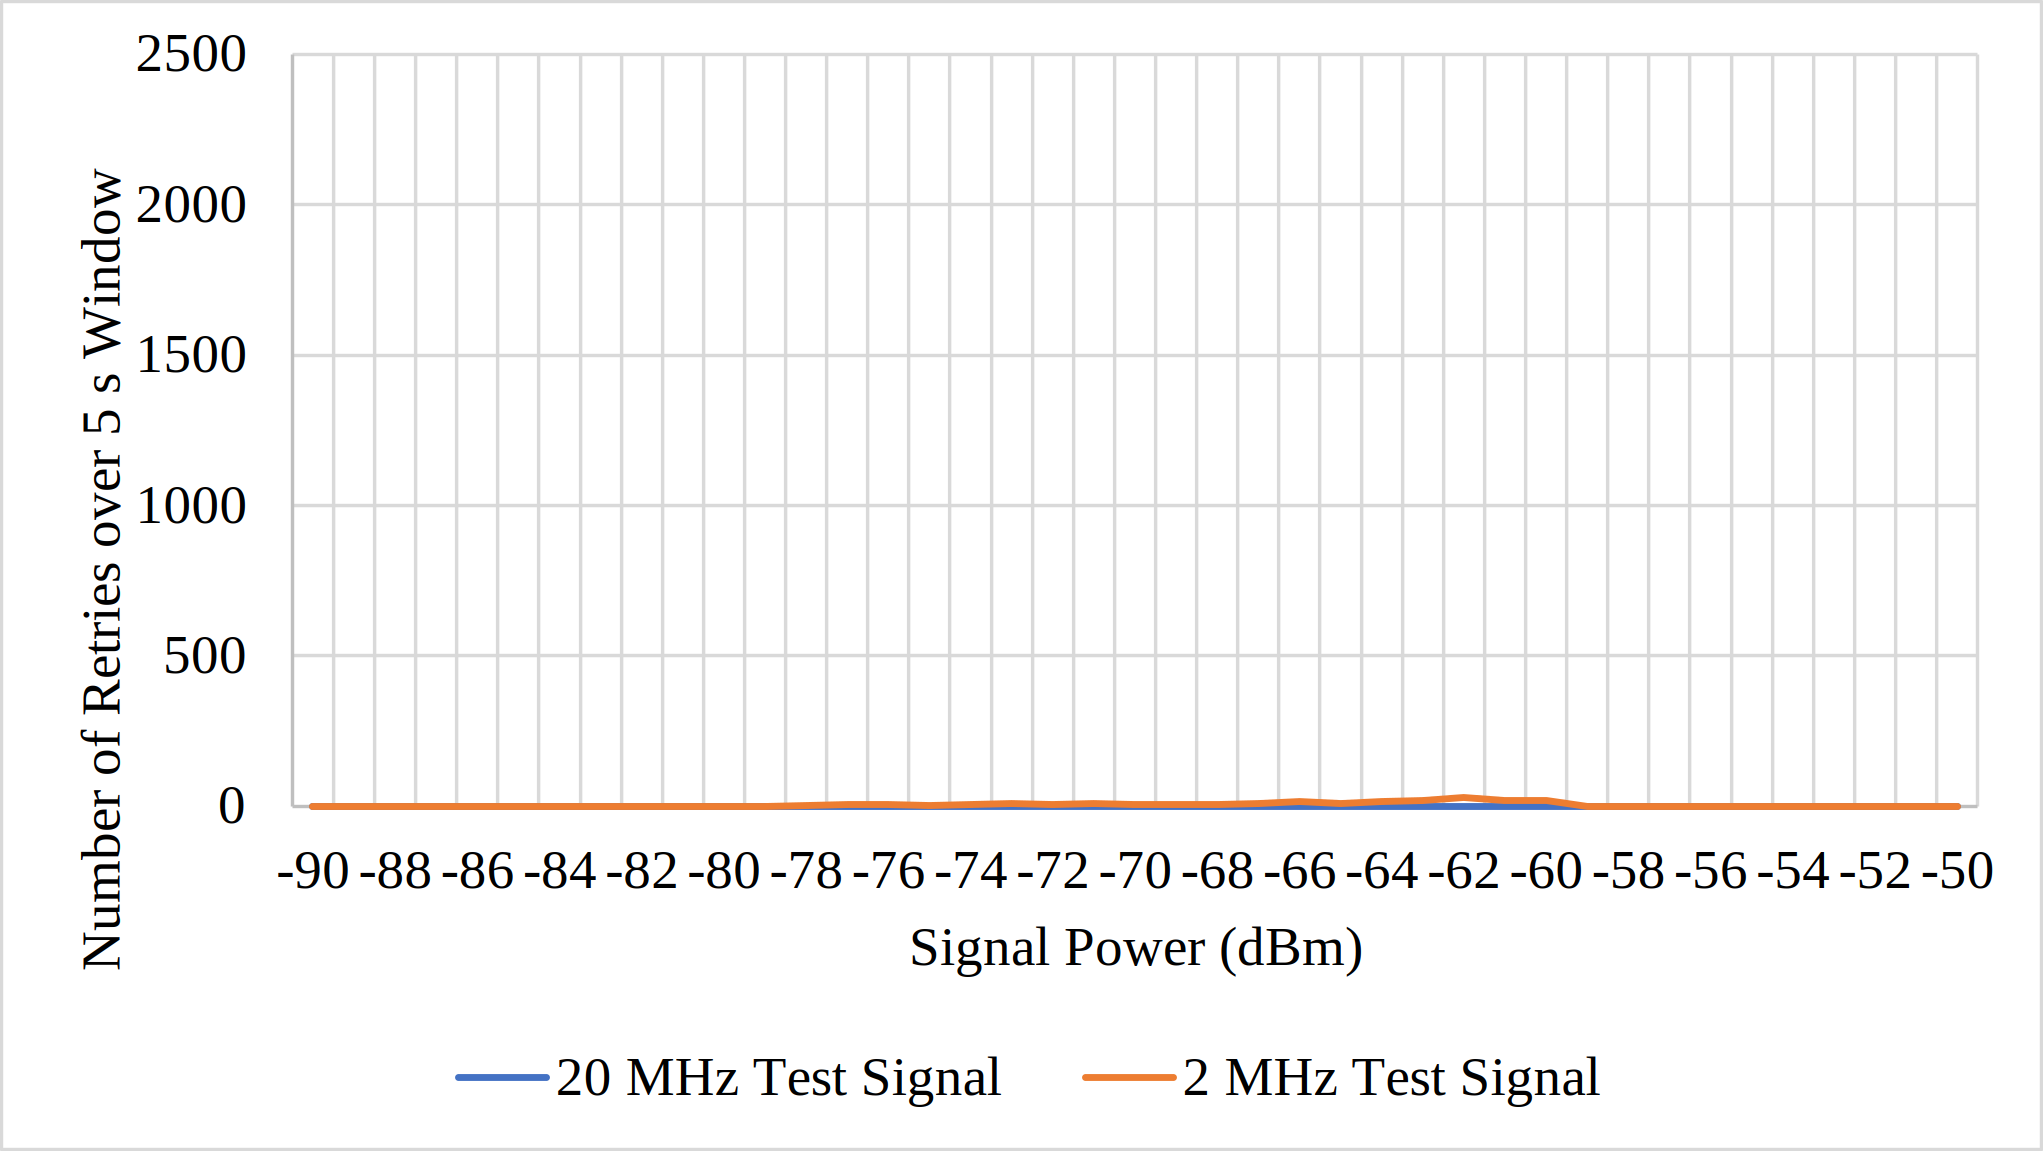
\includegraphics[width=8cm]{EDT_Retries.png}
        \centering
        \caption{EDT Test - Data packet retries vs. 20 and 2 MHz Gaussian signals (DUT-1)}
        \label{pic:Cisco_EDT_Retries_Default}
    \end{figure}

From Fig. \ref{pic:Cisco_EDT_TP_Default}, it is evident that the \ac{edt} of DUT-1 is inconsistent between a \SI{20}{\mega\hertz} and \SI{2}{\mega\hertz} signal. In response to a a \SI{20}{\mega\hertz} signal, throughput ceases around a signal power of \SI{-55}{\dBm}, compared to a signal power of \SI{-58}{\dBm} for a \SI{2}{\mega\hertz} signal. Furthermore, the results in Fig. \ref{pic:Cisco_EDT_Retries_Default} indicate that the throughput loss observed in response to a narrowband test signal is due to transmission throttling and not packet corruption as there is not a proportional increase in the number of data packet retries to accompany the decline in throughput. This correlation between throughput and the number of retries is found to hold for all further DUT-1 results presented in this section, and is only shown for this first set of results for the sake of brevity. This discrepancy in the response to wideband and narrowband signals indicates that the DUT does not measure energy over the channel in as absolute of a manner such as a signal analyzer. This could be due to the fact that NB FH traffic is not permitted in \SI{5}{\giga\hertz}, nevertheless, such \ac{lbt} mechanisms might need to be refined in \SI{6}{\giga\hertz} to account for these types of traffic.

From Fig. \ref{pic:Netgear_EDT_TP_Default}, it is evident that the \ac{edt} of DUT-2 is inconsistent between a \SI{20}{\mega\hertz} and \SI{2}{\mega\hertz} signal. In response to a a \SI{20}{\mega\hertz} signal, throughput ceases around a signal power of \SI{-58}{\dBm}, compared to a signal power of \SI{-56}{\dBm} for a \SI{2}{\mega\hertz} signal. As with DUT-1, this inconsistency is likely a result of measurement inaccuracy in response to narrowband signaling. Furthermore, DUT-2 is noticeably less sensitive to a \SI{2}{\mega\hertz} signal in direct contrast to the behaviour of DUT-1. The implications of this on coexistence are evident, in that Wi-Fi devices might be disproportionately affected by a narrowband signal due to their own internal measurement procedures, and that implementation of \ac{lbt} varies from vendor to vendor, despite the IEEE 802.11-2020 standard being explicit about an absolute measurement threshold.

Following this baseline test, one concern that arises is the null DC sub-carrier which could impact channel measurements of narrowband signals at the centre of the channel. Furthermore, NB FH devices will not always hop onto the same frequency inside the Wi-Fi channel, and thus it is important to assess Wi-Fi's ability to perform \ac{lbt} on the signal at different frequencies within the channel.  The next test is to transmit \SI{2}{\mega\hertz} signal at different carrier frequencies within the channel by modifying the centre frequency of the SDR. Offsets are given in MHz, and only the positive range of frequencies is evaluated due to the sub-carrier symmetry across the center frequency. The results are displayed in Fig. \ref{pic:Cisco_EDT_Offset} and \ref{pic:Netgear_EDT_Offset}.
\begin{figure}[h]
        \includegraphics[width=8cm]{EDT_fc_offset_Cisco.png}
        \centering
        \caption{EDT Test - Wi-Fi throughput vs. 2 MHz Gaussian signals at varying offsets from 5180 MHz (DUT-1)}
        \label{pic:Cisco_EDT_Offset}
    \end{figure}
\begin{figure}[hb]
        \includegraphics[width=8cm]{EDT_fc_offset_Netgear.png}
        \centering
        \caption{EDT Test - Wi-Fi throughput vs. 2 MHz Gaussian signals at varying offsets from 5180 MHz (DUT-2)}
        \label{pic:Netgear_EDT_Offset}
    \end{figure}


The results in Fig. \ref{pic:Cisco_EDT_Offset} and \ref{pic:Netgear_EDT_Offset} both demonstrate that \ac{lbt} performance varies depending on what frequency the \SI{2}{\mega\hertz} signal is transmitted. Most noticeably, performance varies most at the edge of the \SI{20}{\mega\hertz} channel on carrier frequency \SI{5189}{\mega\hertz}. DUT-1 is about \SI{3}{\dB} less sensitive to the narrowband signal at this frequency as the throughput ceases at \SI{-56}{\dBm} instead of \SI{-58}{\dBm}, and DUT-2 does not perform \ac{lbt} at all in the presence of this signal even up to a signal power of \SI{-50}{\dBm}. The implications of this show that DUT-2 most likely has a superior out-of-band filter as the majority of this signal's energy would reside outside of the occupied channel bandwidth, which is only about \SI{16.6}{\mega\hertz} after accounting for factors such as the guard intervals.


In addition to observing behaviour at the channel edge, it is also important to observe behavioural discrepancies at the channel centre. Given that in the IEEE 802.11a OFDM floorplan, there is a null tone at DC, energy measurement may differ at this frequency compared to other parts of the channel.  DUT-2 appears to be less sensitive by roughly \SI{4}{dB} at the center frequency where there is a null tone. In contrast, DUT-1 is able to perform \ac{cca} at this center frequency notch just as well as at other carrier frequencies within the channel. This again indicates a difference in implementation of energy detection within these devices.

To gain further insight into the ability to perform \ac{lbt} at various sub-carrier, a \SI{312.5}{\kilo\hertz} Gaussian signal is transmitted from the SDR as this is the sub-carrier spacing defined in the IEEE 802.11a standard. This very narrow signal is transmitted at the channel's center frequency, the frequency of a data tone, the frequency of a pilot tone, and \SI{312.5}{\kilo\hertz} to the right of the last sub-carrier in the OFDM sub-carrier arrangement. The results are shown in Fig. \ref{pic:Cisco_subcarrier_edt} and \ref{pic:Netgear_subcarrier_edt}.

\begin{figure}[h]
        \includegraphics[width=8cm]{Cisco_312_edt.png}
        \centering
        \caption{EDT Test - Wi-Fi throughput vs. 312.5 kHz Gaussian signals at select sub-carrier frequencies (DUT-1)}
        \label{pic:Cisco_subcarrier_edt}
    \end{figure}
\begin{figure}[h]
        \includegraphics[width=8cm]{Netgear_312_edt.png}
        \centering
        \caption{EDT Test - Wi-Fi throughput vs. 312.5 kHz Gaussian signals at select sub-carrier frequencies (DUT-2)}
        \label{pic:Netgear_subcarrier_edt}
    \end{figure}
From Fig. \ref{pic:Cisco_subcarrier_edt}, it is evident that DUT-1 performs \ac{lbt} equivalently at a null, data sub-carrier and pilot tone, and is unable to measure a signal outside its occupied bandwidth with as much accuracy. On the other hand, from Fig. \ref{pic:Netgear_subcarrier_edt}, DUT-2 is unable to measure any of these signals as accurately as the \SI{20}{\mega\hertz} and \SI{2}{\mega\hertz} signals previously used, and does not perform \ac{lbt} outside its occupied channel bandwidth as expected. This discrepancy in device behaviour serves to further validate the notion that energy measurement is highly vendor dependent in terms of implementation.

As mentioned, NB FH is a permitted mode of operation in \SI{6}{\giga\hertz}. While the insights gained from using static signals with a maximum duty cycle are important for understanding the baseline \ac{lbt} behaviour of these IEEE 802.11 devices, some form of dynamic transmission needs to be studied. Thus, to gauge the impact of dynamic traffic, a \SI{2}{\mega\hertz} Gaussian signal with 10\%  and 50\% duty cycles and varying dwell times is inserted onto the channel at \SI{5180}{\mega\hertz}. In addition, the frequency hopping algorithm described in Section IV Part B, which has a \SI{7.5}{\milli\second} dwell time and 10\% in-channel duty cycle is assessed along with the non-hopping 10\% duty cycle signals. The power level of the signal is fixed to above the experimental \ac{edt} of the two DUTs found from the baseline tests. This is done to ensure that when the signal is present in the channel, the IEEE 802.11 DUT should perform \ac{lbt}. The results for each device are shown in Fig. \ref{pic:Cisco_dynamic_edt} and \ref{pic:Netgear_dynamic_edt}.

\begin{figure}[ht]
        \includegraphics[width=8cm]{dynamic_edt_10.png}
        \centering
        \caption{EDT Test - Wi-Fi throughput vs. Gaussian signals with 10\% duty cycle and varying dwell times}
        \label{pic:Cisco_dynamic_edt}
    \end{figure}
\begin{figure}[ht]
        \includegraphics[width=8cm]{dynamic_edt_50.png}
        \centering
        \caption{EDT Test - Wi-Fi throughput vs. Gaussian signals with 50\% duty cycle and varying dwell times}
        \label{pic:Netgear_dynamic_edt}
    \end{figure}
    
Recalling that the nominal throughput is set to 90\%, the expected throughput for a signal with 10\% and 50\% duty cycles would be 81\%  and 45 \% respectively. The results for both DUTs show that this expected throughput is achieved if not surpassed for almost all combinations of dwell-times and duty-cycles tested. The only exception to this is a \SI{100}{\micro\second} dwell time signal with 50\% duty cycle on DUT-1, where the throughput is lower than expected. One reason for this outlier could be due to the random backoff implementation of the device. It can also be seen that DUT-1 slightly under performs compared to DUT-2 in almost all test cases. As discussed, DUT-1 is more sensitive to a \SI{2}{\mega\hertz} Gaussian signal than DUT-2, which could attribute to the discrepancy observed here. In addition, the results of \cite{4215723} demonstrate a differing implementations of backoff across six commercial Wi-Fi cards, which is another likely explanation for this observed discrepancy.

\subsection{Insertion of Gaussian Signal to Wi-Fi Receiver}
In the previous section, the SDR transmission is sent to the Wi-Fi transmitter which is expected to perform \ac{lbt} in response to any signal on the channel. In addition to this, it is important to assess the impacts of interference on Wi-Fi's ability to correctly receive and decode packets. Thus, in this section, the SDR transmission is sent to the Wi-Fi receiver which is not expected to perform \ac{lbt}, allowing the impact of interference to be directly abstracted from the throughput. 

Similar to the previous section, a baseline test is conducted by transmitting wideband and narrowband signals from the SDR onto the centre frequency of the Wi-Fi channel in an ongoing Wi-Fi link and observing the throughput. These are shown in Fig. \ref{pic:Cisco_rx_tp} and \ref{pic:Netgear_rx_tp}.
\begin{figure}[hb]
        \includegraphics[width=8cm]{Cisco_rx_tp.png}
        \centering
        \caption{Reception Test - Wi-Fi throughput vs. 20 and 2 MHz Gaussian signals (DUT-1)}
        \label{pic:Cisco_rx_tp}
    \end{figure}

\begin{figure}[ht]
        \includegraphics[width=8cm]{Netgear_rx_tp.png}
        \centering
        \caption{Reception Test - Wi-Fi throughput vs. 20 and 2 MHz Gaussian signals (DUT-2)}
        \label{pic:Netgear_rx_tp}
    \end{figure}
As with the tests from Part A, the number of data packet retries in a 5 second interval is also collected on DUT-1 to corroborate the primary reason for throughput loss. This is shown in Fig. \ref{pic:cisco_retries}.
\begin{figure}[ht]
        \includegraphics[width=8cm]{rx_retries.png}
        \centering
        \caption{Reception Test - Data packet retries vs. 20 and 2 MHz Gaussian signals (DUT-1)}
        \label{pic:cisco_retries}
    \end{figure}


In the presence of the \SI{20}{\mega\hertz} signal, both devices are impacted relatively the same: the connection becomes unreliable at \SI{-58}{\dBm} which is \SI{8}{\dB} above the fixed Wi-Fi signal power at the receiver. However, their behavior to a \SI{2}{\mega\hertz} signal shows more variation in the impact on throughput. DUT-1 loses a reliable connection around a signal power of \SI{-62}{\dBm}, whereas DUT-2 loses a reliable connection around a signal power of \SI{-53}{\dBm}. This discrepancy indicates variation in the implementation of the receiver design, showing that the resiliency to narrowband technology can vary from vendor to vendor. In addition, the number of data packet retries on DUT-1 increases proportionally with the interference power, indicating that packet corruption is the primary reason for the decline in throughput, and not \ac{lbt}. This correlation between the throughput and the data retries continues for all DUT-1 results presented in this section.

Again, since the NB FH signals are not always going to active at the same frequency in the channel, the next test is to transmit \SI{2}{\mega\hertz} signal at different carrier frequencies within the Wi-Fi channel by modifying the centre frequency of the SDR. Offsets are given in MHz, and only the positive range of frequencies is evaluated due to the sub-carrier symmetry across the center frequency. The results are displayed in Fig. \ref{pic:Cisco_rx_offset} and \ref{pic:Netgear_rx_offset}.
\begin{figure}[hb]
        \includegraphics[width=8cm]{Offset_rx_cisco.png}
        \centering
        \caption{Reception Test - Wi-Fi throughput vs. 2 MHz Gaussian signal at varying offsets from 5180 MHz (DUT-1)}
        \label{pic:Cisco_rx_offset}
    \end{figure}
\begin{figure}[t]
        \includegraphics[width=8cm]{Offset_rx_Netgear.png}
        \centering
        \caption{Reception Test - Throughput vs. 2 MHz Gaussian signal at varying offsets from 5180 MHz (DUT-2)}
        \label{pic:Netgear_rx_offset}
    \end{figure}
From these results, it seems that the impact of the narrowband transmission on the Wi-Fi throughput does indeed vary at different frequencies within the channel. In the case of DUT-1, it is most susceptible to the signal at \SI{5186}{\mega\hertz} and least susceptible to the signal at the edge frequencies of the channel. This discrepancy is most likely due to which specific combination of sub-carriers are being impacted and how that impacts both the data and the channel estimation procedures. For DUT-2, it is most susceptible to interference at \SI{5188}{\mega\hertz} and least susceptible at the channel edge of \SI{5189}{\mega\hertz} again supporting the assumption that DUT-2 has a better out-of-band rejection filter. It is also relatively robust against a transmission at the centre frequency of \SI{5180}{\mega\hertz}, which is interesting to note given the presence of a null at DC. Despite adherence to standardized physical layer processes as defined by the IEEE 802.11a standard, discrepancies are observed in the performance of devices from different vendors when subjected to a \SI{2}{\mega\hertz} interference signal. These variations in behavior could be attributed to differences in RF front-end design, receiver sensitivity and selectivity, proprietary signal processing algorithms, and hardware quality, all of which influence a device's ability to manage narrowband interference. Such disparities highlight the impact of implementation-specific factors, beyond the standardized PHY specifications, on the real-world performance and interference resilience of Wi-Fi devices.

As discussed, interference at different frequencies within the channel show different effects. Thus, a \SI{312.5}{\kilo\hertz} signal is transmitted over the SDR at the centre frequency of the channel, at the frequency of a data tone, and at the frequency of a pilot tone to gauge the varying degrees of impact. The results are shown in Fig. \ref{pic:Cisco_312_rx} and \ref{pic:Netgear_312_rx}.
\begin{figure}[ht]
        \includegraphics[width=8cm]{Cisco_312_rx.png}
        \centering
        \caption{Reception Test - Wi-Fi throughput vs. 312.5 kHz Gaussian signal at select sub-carrier frequencies (DUT-1)}
        \label{pic:Cisco_312_rx}
    \end{figure}
\begin{figure}[b]
        \includegraphics[width=8cm]{Netgear_312_rx.png}
        \centering
        \caption{Reception Test - Wi-Fi throughput vs. 312.5 kHz Gaussian signal at select sub-carrier frequencies (DUT-2)}
        \label{pic:Netgear_312_rx}
    \end{figure}
In the case of DUT-1, it appears that interfering with a pilot tone is the most damaging, compared with transmitting the signal at a null which is the least damaging as expected. Since pilot tones serve to estimate the channel, interfering with one of these could have a wider-spread impact than interfering with a data tone which can be accounted for by error-correction mechanisms. The discrepancy is less distinct in DUT-2, again potentially due to different implementations. Nonetheless, a similar trend is observed.

Finally, the impact of dynamic interference on Wi-Fi reception is assessed using 10\% duty cycle \SI{2}{\mega\hertz} interference with varying dwell-times, and using the frequency hopping algorithm described in Section IV Part B. The results are displayed in Fig. \ref{pic:Cisco_rx_dynamic} and \ref{pic:Netgear_rx_dynamic}.
\begin{figure}[ht]
        \includegraphics[width=8cm]{Rx_Cisco_dynamic.png}
        \centering
        \caption{Reception Test - Wi-Fi throughput vs. Dynamic 2 MHz interference (DUT-1)}
        \label{pic:Cisco_rx_dynamic}
    \end{figure}
\begin{figure}[ht]
        \includegraphics[width=8cm]{Rx_Netgear_dynamic.png}
        \centering
        \caption{Reception Test - Throughput vs. Dynamic 2 MHz interference (DUT-2)}
        \label{pic:Netgear_rx_dynamic}
    \end{figure}

In both cases, it is evident that longer dwell-times lead to better throughput for the test case assessed. To understand why this might be, we should observe the impact on the over the air (OTA) transmission of packets.

Given that the best achievable data rate is \(6\) Mb/s with a UDP packet size of \(1470\) B, the amount of time a packet is on the air can be calculated. Converting the packet size to bits:
\[ 1470 \text{ B/pkt} = 11760 \text{ b/pkt} \]

To calculate the corresponding packet transmission rate:
\[ \text{Packet rate} = \frac{6 \times 10^6 \text{ b/s}}{11760 \text{ b/pkt}} = 510.2 \text{ pkt/s} \]

Inversely, it takes roughly \SI{2}{\milli\second} to transmit a single packet over the air. Therefore, the number of packets interfered with in one period of the interference signal will vary proportionately with its dwell time. A \SI{100}{\micro\second} dwell-time signal will interfere with a fraction of every packet, whereas, a \SI{7.5}{\milli\second} dwell-time signal will interfere with a short stream of packets, then leave a longer stream uninterfered with. The latter case appears to be less detrimental to an ongoing Wi-Fi connection.

\section{Conclusion}
This study offers a comprehensive experimental evaluation of Wi-Fi's coexistence capabilities when operating alongside other wideband and narrowband signals, particularly NB FH signals. By leveraging a novel methodology that integrates off-the-shelf IEEE 802.11 devices with software-defined radio (SDR) technology, we are able to transmit pre-calculated signals with desired PHY and MAC layer properties without device modification. Our measurements, conducted on both the transmitter and receiver sides, assess the efficacy of Listen Before Talk (LBT) and the resilience of devices to various interference types.

The results reveal significant variations in device behavior between the two devices under test (DUTs), originating from different manufacturers, despite adherence to standardized requirements. This manufacturer-dependent variation in implementation warrants further investigation, especially in the context of ensuring harmonious coexistence within the \SI{6}{\giga\hertz} band. Additionally, this study underscores the vital role of experimental research in verifying simulated results and theoretical predictions, ultimately contributing to a more robust understanding of coexistence dynamics in real-world scenarios.



\section*{Acknowledgments}
The funding for this research has been provided by Ericsson, and Natural Sciences and Engineering Research Council of Canada (NSERC). Additionally, we would like to thank Dr. Guido Hiertz from Ericsson Germany for his valuable insights, comments, and suggestions.

\bibliographystyle{IEEEtran}
\bibliography{IEEEabrv,main}

\clearpage
\appendices
\section*{Appendix}

\begin{figure}[h]
    \includegraphics[width=8cm]{Inside_chamber.jpg}
    \centering
    \caption{Testbed components inside RF isolation chamber.}
    \label{pic:testbed_1}
\end{figure}
\begin{figure}[h]
    \includegraphics[width=8cm]{Signal_analyzer.jpg}
    \centering
    \caption{Signal analyzer.}
    \label{pic:testbed_2}
\end{figure}

\begin{figure}[h]
    \includegraphics[width=8cm]{Outside_chamber.jpg}
    \centering
    \caption{Testbed components outside RF isolation chamber.}
    \label{pic:testbed_3}
\end{figure}



\end{document}